\documentclass[11pt,a4paper]{article}
\usepackage[T1]{fontenc}
\usepackage[utf8]{inputenc}
\usepackage{mathptmx}
\usepackage[margin=2.3cm]{geometry}
\usepackage{amsmath,amssymb,amsthm,mathtools,bm}
\usepackage{booktabs,multirow,array}
\usepackage{microtype}
\usepackage{xcolor}
\usepackage{graphicx}
\usepackage{caption}
\usepackage{float}
\usepackage{pgfplots}
\pgfplotsset{compat=1.17}
\usepackage[colorlinks=true,linkcolor=navy,citecolor=navy,urlcolor=navy]{hyperref}
\usepackage{cleveref}

\definecolor{navy}{HTML}{1E2761}
\definecolor{cblue}{HTML}{3A4FA0}
\definecolor{camber}{HTML}{C9821E}
\definecolor{cgreen}{HTML}{2E9E6B}
\definecolor{cred}{HTML}{C0392B}
\captionsetup{font=small,labelfont=bf}

\newtheorem{proposition}{Proposition}
\newtheorem{definition}{Definition}
\theoremstyle{remark}
\newtheorem{remark}{Remark}
\newcommand{\repourl}{\url{https://github.com/MDP2004/MuST-Walk}}
\newcommand{\R}{\mathbb{R}}
\newcommand{\E}{\mathbb{E}}
\newcommand{\tH}{\widetilde{H}}
\DeclareMathOperator{\AP}{AP}

\title{\textbf{MuST-Walk: Efficient Temporal Link Prediction with Multi-Scale Temporal Walk Encodings}\\[4pt]
\large DAL 518: Graph Machine Learning, Project 4.3}
\author{Abhi Raj (23125003) \and Manas Dnyaneshvar Patil (23125020) \and Kamranjeet Singh (23125016)}
\date{November 2026\\[3pt]\normalsize Code and results: \repourl}

\begin{document}
\maketitle

\begin{abstract}
TPNet encodes temporal walks with a random-projection sketch that uses one exponential decay rate per dataset. We proposed MuST-Walk (Multi-Scale Temporal Walks): several decay rates sharing one projection, combined by a learned fusion gate. We implemented it with exact tests against brute-force walk enumeration, then inspected the data and the pipeline before spending compute. That audit found a same-timestamp information leak in the sketch, random negatives that are true edges for 8.3--95.7\% of draws on yearly data, and truncated training in our own early runs. We then reran everything on corrected code: 232 pre-registered runs on six DyGLib and four TGB datasets, about 535 compute-hours, all finished. Multi-scale sketches improve the historical-negative score on 3 of 6 DyGLib datasets, specifically where the tuned decay erases the previous time step, and they are not a general improvement. Training on historical negatives gives the largest gain on all six datasets (+9.44 to +25.62 AP, 18 of 18 seeds), at a cost on random-negative tests and with mixed results on TGB. We also derive why the update rule carries a positive exponent while the walk score decays, restore the $O(k\,d_R)$ per-edge cost with a lazy update (24 times faster at $10^6$ nodes), prove a ceiling on random-negative AP, and show that on UN Trade and UN Vote a direction-aware recency rule beats every model we trained.
\end{abstract}

\section{Introduction}
A continuous-time dynamic graph is a stream of timestamped edges $\mathcal{G}=\{(u_i,v_i,t_i)\}$ with $t_1\le t_2\le\dots$. Temporal link prediction asks, at time $t$, whether $u$ and $v$ will interact. The strongest signals are recency and frequency of connection, and temporal walks capture both.

Lu et al.\ \cite{tpnet} showed that many relative encodings are choices of a walk score and a readout, and that a temporal walk matrix can be maintained implicitly through a random projection. TPNet has one limitation we set out to address: a single decay rate $\lambda$ per dataset forces short and long ranges to share one scale. On yearly data the tuned value leaves no usable memory at all. At $\lambda=10^{-5}$ with timestamps in seconds, one year contributes a factor of $e^{-315}\approx 10^{-137}$.

Our contributions are:
\begin{itemize}\itemsep1pt
\item MuST-Walk: $J$ sketches that share one projection, with concatenation, average and gated residual fusion (\cref{sec:method}).
\item A derivation that reconciles the positive exponent in the TPNet update with the negative exponent in the walk score, and a lazy update that achieves the $O(k\,d_R)$ per-edge bound in practice (\cref{sec:sign,sec:lazy}).
\item A data and pipeline audit, including a provable ceiling on random-negative AP (\cref{sec:data}).
\item A pre-registered evaluation of 232 runs, with reasons for each outcome, separated into measured and likely (\cref{sec:results,sec:why}).
\end{itemize}

\section{Background}
\subsection{Temporal walks and the TPNet score}
\begin{definition}[Temporal walk score]
A $k$-step temporal walk $W=[(w_0,t_0),\dots,(w_k,t_k)]$ has strictly decreasing times $t_0>t_1>\dots>t_k$ and consecutive nodes joined by an interaction at the later of the two times. TPNet scores it at time $t$ by
\begin{equation}
s(W)=\prod_{i=1}^{k} e^{-\lambda(t-t_i)},\qquad \lambda\ge 0.
\end{equation}
\end{definition}
The temporal walk matrix $A^{(l)}(t)\in\R^{n\times n}$ has entries $A^{(l)}_{u,w}(t)=\sum_{W\in\mathcal{W}^{(l)}(u,w,t)}s(W)$, with $A^{(0)}=I$.

\subsection{The sketch}
Let $P\in\R^{n\times d_R}$ have independent $\mathcal{N}(0,1/d_R)$ entries. TPNet keeps $H^{(0)}=P$, $H^{(1)},\dots,H^{(k)}\in\R^{n\times d_R}$, initially zero for $l\ge 1$, and on interaction $(u,v,t)$ it applies for $l=k,\dots,1$:
\begin{equation}\label{eq:update}
H_u^{(l)}\leftarrow H_u^{(l)}+e^{\lambda t}H_v^{(l-1)},\qquad H_v^{(l)}\leftarrow H_v^{(l)}+e^{\lambda t}H_u^{(l-1)} .
\end{equation}
Theorem 1 of \cite{tpnet} states $e^{-\lambda l t}H^{(l)}(t)=A^{(l)}(t)P$ when all timestamps differ, and Theorem 2 gives a Johnson--Lindenstrauss guarantee \cite{jl} on inner products when $d_R\ge 24\,\varepsilon^{-2}\log\bigl(4^{1/3}(k+1)n\bigr)$. For a pair $(u,v)$ the model forms the matrix of inner products among $\{r_u^{(l)},r_v^{(l)}\}_{l=0}^{k}$, a pairwise feature of dimension $D=(2k+2)^2$, and passes it with neighbour and time information to an MLP-Mixer encoder and a link predictor.

\subsection{Why the update has a positive sign}\label{sec:sign}
Equation~\eqref{eq:update} looks wrong at first sight, since a decay should carry a negative exponent for positive $\lambda$. The sign is correct, but only because the stored $H^{(l)}$ is not the decayed quantity. The decayed quantity is $\tH^{(l)}(t):=e^{-\lambda l t}H^{(l)}(t)$.

\begin{proposition}[Equivalence of the two forms]\label{prop:sign}
The update \eqref{eq:update} is equivalent to the decay-form recursion
\begin{align}
\tH^{(l)}(t') &= e^{-\lambda l (t'-t)}\,\tH^{(l)}(t) && \text{between events, } t'>t, \label{eq:decay}\\
\tH_u^{(l)}(t^{+}) &= \tH_u^{(l)}(t)+\tH_v^{(l-1)}(t) && \text{at an event } (u,v,t). \label{eq:event}
\end{align}
\end{proposition}
\begin{proof}
Between events $H^{(l)}$ is constant, so $\tH^{(l)}(t')=e^{-\lambda l t'}H^{(l)}=e^{-\lambda l(t'-t)}e^{-\lambda l t}H^{(l)}$, which is \eqref{eq:decay}. At an event, multiply \eqref{eq:update} by $e^{-\lambda l t}$:
$\tH_u^{(l)}(t^{+})=\tH_u^{(l)}(t)+e^{-\lambda l t}e^{\lambda t}H_v^{(l-1)}(t)=\tH_u^{(l)}(t)+e^{-\lambda(l-1)t}H_v^{(l-1)}(t)=\tH_u^{(l)}(t)+\tH_v^{(l-1)}(t)$.
\end{proof}
For $l=1$ the point is visible in one line. After edges $(u,v_i,t_i)$, we have $H_u^{(1)}(T)=\sum_i e^{\lambda t_i}P_{v_i}$, so
\begin{equation}
e^{-\lambda T}H_u^{(1)}(T)=\sum_i e^{-\lambda(T-t_i)}P_{v_i}.
\end{equation}
Old edges are not shrunk when stored; new edges are inflated relative to them, and the readout divides by the current inflation. This is the forward-decay construction of Cormode et al.\ \cite{forward}.

The positive form cannot be run directly on our data: UN Vote spans about 72 years, so $\lambda t\approx 2.3\times10^{4}$ at $\lambda=10^{-5}$, while a double overflows at $e^{709}$. The authors' code therefore uses the decay form (\ref{eq:decay}--\ref{eq:event}), multiplying by $\exp(-\lambda\Delta)^{l}$. That choice has a complexity cost, which \cref{sec:lazy} removes.

\section{MuST-Walk}\label{sec:method}
\subsection{Multi-scale sketching}
Choose rates $\lambda_1,\dots,\lambda_J$ and maintain $H_j^{(l)}$ for each, with a single shared $H_j^{(0)}=P$. Rates spread around the tuned rate $\lambda^\star$ and include no decay: $\{10\lambda^\star,\lambda^\star,\lambda^\star/10,0\}$ on UCI and Enron, and $\{10^{-5},10^{-7},2.2\times10^{-8},0\}$ on yearly data (five rates on US Legis., which adds $10^{-6}$). Since \eqref{eq:update} is linear and each scale runs it unchanged, Theorem 1 holds per scale and adds no new approximation. A union bound over $J$ scales changes the JL requirement only to $d_R\ge 24\,\varepsilon^{-2}\log\bigl(4^{1/3}J(k+1)n\bigr)$.

\subsection{Why one shared projection}
Sharing $P$ saves $J-1$ copies of $n\,d_R$ numbers, and it is also what makes comparison across scales meaningful.
\begin{proposition}[Cross-scale inner products]\label{prop:cross}
Let $r_u^{(l)}(\lambda)=A_{\lambda}^{(l)}(t)[u,:]\,P$. With one shared $P$,
\begin{equation}
\E\bigl\langle r_u^{(l)}(\lambda_a),\,r_v^{(m)}(\lambda_b)\bigr\rangle = \sum_{w} A^{(l)}_{\lambda_a}[u,w]\;A^{(m)}_{\lambda_b}[v,w],
\end{equation}
a sum over shared intermediate nodes that weights $u$'s walks at rate $\lambda_a$ and $v$'s at rate $\lambda_b$. With independent projections $P_a,P_b$ the expectation is $0$.
\end{proposition}
\begin{proof}
$\langle r_u,r_v\rangle=A_{\lambda_a}^{(l)}[u,:]\,PP^{\top}A_{\lambda_b}^{(m)}[v,:]^{\top}$ and $\E[PP^{\top}]=I$ since $\E[\sum_c P_{wc}P_{w'c}]=\mathbb{1}[w=w']$. For independent zero-mean projections $\E[P_aP_b^{\top}]=0$.
\end{proof}

\subsection{Fusion}
Let $f_1,\dots,f_J\in\R^D$ be the per-scale pairwise features and $f_b$ the base scale at the tuned rate. The gated residual model is
\begin{equation}\label{eq:gate}
f=f_b+\beta\sum_{j=1}^{J}\alpha_j f_j,\qquad \alpha=\mathrm{softmax}\bigl(g_\phi([f_1,\dots,f_J])\bigr),\quad \beta_0=0,
\end{equation}
so that training starts exactly at TPNet. Fixed average sets $\alpha_j=1/J$. Concatenation, $f=[f_1,\dots,f_J]\in\R^{JD}$, is the simplest option. In early experiments the gate underperformed and was unstable (\cref{tab:oldabl}), so we made concatenation the main configuration, kept gate and average as ablations, and moved our remaining effort to the directions below.

\subsection{Further configurations}
\paragraph{Cross-scale features (MuST-Cross).} Concatenation plus the $J(J-1)(k+1)^2$ inner products between different scales from \cref{prop:cross}, log-scaled and passed through a small MLP. This needs no extra sketch state.
\paragraph{Equal memory (MuST-Equal).} $d_R/J$ per scale, so total state equals TPNet's.
\paragraph{Strict time.} See \cref{sec:strict}.
\paragraph{Historical-negative training (-HN).} Normally every fake training pair is random, so the model can succeed by learning that familiar pairs are real. We replace about half of the fakes with pairs seen strictly before the batch and not active in its time interval, and we choose the best epoch on historical validation. Historical negatives follow Poursafaei et al.\ \cite{poursafaei}. Similar training strategies appear in ENS \cite{ens}, CurNM \cite{curnm} and ATNSF \cite{atnsf}, so this is not a new idea. On TGB, validation stays on TGB's fixed negatives.
\paragraph{Learned decay.} Treating $\log\lambda$ as a parameter with exact forward-mode gradients, tested as a separate experiment.

\section{Complexity}\label{sec:lazy}
\subsection{The per-edge bound and the decay-form code}
The stored form \eqref{eq:update} touches $2k$ vectors per edge, hence $O(k\,d_R)$ per edge. The decay form must apply \eqref{eq:decay} to \emph{every} node before each batch, because every row ages. For $b$ edges per batch the cost is
\begin{equation}
T_{\text{eager}}=O\bigl(J\,k\,d_R\,(n+b)\bigr)\ \text{per batch}\quad\Longrightarrow\quad O\bigl(J\,k\,d_R\,(1+n/b)\bigr)\ \text{per edge},
\end{equation}
which grows with $n$ and contradicts the advertised bound.

\subsection{Lazy update}
Store $\hat H^{(l)}$ and one scalar $c_l$ per layer, with the invariant $\tH^{(l)}=c_l\,\hat H^{(l)}$. Moving time forward by $\Delta$ sets $c_l\leftarrow c_l\,e^{-\lambda l\Delta}$, which is $O(1)$ per layer. An event adds $\tH_v^{(l-1)}$ to $\tH_u^{(l)}$, that is
\begin{equation}
\hat H_u^{(l)}\leftarrow \hat H_u^{(l)}+\frac{c_{l-1}}{c_l}\,\hat H_v^{(l-1)},\qquad \frac{c_{l-1}}{c_l}=e^{+\lambda\,(t-t_0)}\ \text{(up to renormalisation)}.
\end{equation}
The positive exponent of \eqref{eq:update} returns here, relative to a moving origin $t_0$. When $c_l<10^{-12}$ the layer is written out and $c_l$ reset to $1$, which keeps values in float32 range. That is a full write of $O(n\,d_R)$, needed once every $\ln(10^{12})/(\lambda l\,\bar\Delta)$ batches, where $\bar\Delta$ is the mean time gap per batch. Between renormalisations the cost is
\begin{equation}
T_{\text{lazy}}=O(J\,k\,d_R)\ \text{per edge, independent of } n .
\end{equation}
Values match the eager form to about $10^{-7}$ in our tests.

\subsection{Full cost table}
\begin{table}[h]\centering\small
\begin{tabular}{lll}
\toprule
Operation & Cost & Note\\
\midrule
Update, eager & $O(Jk\,d_R(1+n/b))$ per edge & official code path\\
Update, lazy & $O(Jk\,d_R)$ per edge & ours; flat in $n$\\
Strict buffer & $O(1)$ amortised per edge & each edge moved once\\
Pairwise feature & $O(J(2k+2)^2 d_R)$ per query & $(2k+2)^2$ inner products per scale\\
MuST-Cross & $O(J^2(k+1)^2 d_R)$ per query & adds $J(J-1)(k+1)^2$ features\\
Sketch state & $(1+Jk)\,n\,d_R$ numbers & $P$ stored once\\
Rebuild from scratch & $O(Jk\,d_R\,E)$ for $E$ edges & what streaming avoids\\
\bottomrule
\end{tabular}
\caption{Time and space. $k$ walk depth, $J$ scales, $n$ nodes, $d_R$ sketch width, $b$ batch size.}
\end{table}

The state formula is exact. With $k=3$, $d_R=160$, $n=10^6$ and float32, it predicts 2,441.4 MiB for $J=1$ and 7,934.6 MiB for $J=4$. We measured 2,441.5 and 7,935.1 MiB.

\subsection{Measured efficiency}
\begin{figure}[h]\centering
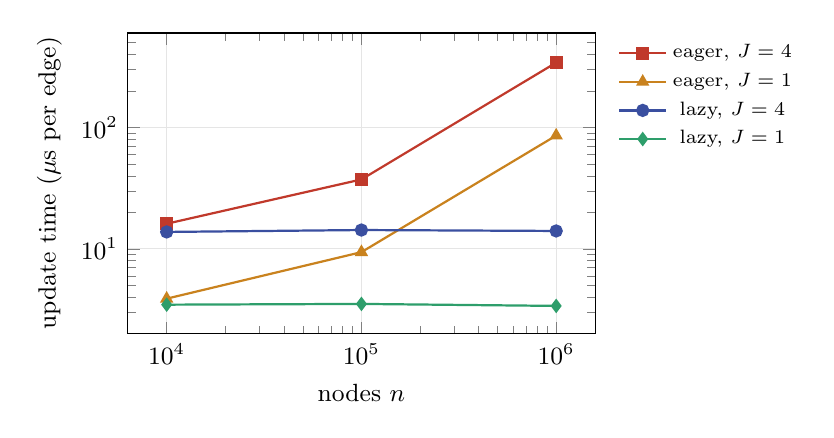
\begin{tikzpicture}
\begin{loglogaxis}[width=0.62\linewidth,height=5.4cm,xlabel={nodes $n$},ylabel={update time ($\mu$s per edge)},
  xtick={10000,100000,1000000},grid=major,grid style={gray!20},legend pos=outer north east,legend style={font=\scriptsize,draw=none},tick label style={font=\small},label style={font=\small},ymin=2,ymax=600]
\addplot[color=cred,mark=square*,thick] coordinates {(10000,16.11)(100000,37.34)(1000000,342.53)};
\addlegendentry{eager, $J=4$}
\addplot[color=camber,mark=triangle*,thick] coordinates {(10000,3.89)(100000,9.40)(1000000,85.84)};
\addlegendentry{eager, $J=1$}
\addplot[color=cblue,mark=*,thick] coordinates {(10000,13.79)(100000,14.30)(1000000,14.05)};
\addlegendentry{lazy, $J=4$}
\addplot[color=cgreen,mark=diamond*,thick] coordinates {(10000,3.47)(100000,3.52)(1000000,3.39)};
\addlegendentry{lazy, $J=1$}
\end{loglogaxis}
\end{tikzpicture}
\caption{Update cost on a Tesla T4, batch size 200. Lazy is flat in $n$ as derived, and eager grows with $n$. At $n=10^6$ and $J=4$ lazy is 24.4 times faster (2.81 vs 68.51 ms per batch). At $n=10^6$ lazy costs 3.4, 7.0, 10.3 and 14.1 $\mu$s per edge for $J=1,\dots,4$, linear in $J$.}\label{fig:lazy}
\end{figure}

On an RTX 6000 Ada with the eager path, $J=1,\dots,4$ at $10^6$ nodes costs 5.0, 10.1, 15.1 and 20.2 ms per batch, with peak GPU memory 3.8 to 14.7 GB. Streaming against a full rebuild at $n=10^5$ and $10^6$ past edges takes 2.47 ms against 11.93 s for $J=4$, a factor of about 4,800.

\section{Opening the data}\label{sec:data}
We opened all six DyGLib datasets and checked the pipeline line by line on two hand-checkable graphs before any new GPU run. tgbl-wiki and tgbl-review were not inspected at the pair level. The sketch was tested against brute-force walk enumeration that shares no code with it (relative error about $10^{-7}$), and 53 unit tests guard the code (19 + 34).

\begin{table}[h]\centering\small\setlength{\tabcolsep}{4pt}
\begin{tabular}{lrrrrrrrr}
\toprule
Dataset & Nodes & Edges & Steps & Tied weight & Random true & Reversed & Active last & Never seen\\
\midrule
US Legis. & 225 & 60,396 & 12 & 96\% & 44.0\% & 12.7\% & 75.6\% & 22.8\%\\
Can. Parl. & 734 & 74,478 & 14 & 98\% & 8.3\% & 1.5\% & 44.1\% & 48.4\%\\
UN Trade & 255 & 507,497 & 32 & 85\% & 59.9\% & 23.2\% & 93.2\% & 0.9\%\\
UN Vote & 201 & 1,035,742 & 72 & 99\% & 95.7\% & 81.0\%$^\dagger$ & 99.9\% & 0.0\%\\
UCI & 1,899 & 59,835 & 58,911 & 0.0\% & 0.1\% & 0.2\% & n/a & 17.9\%\\
Enron & 184 & 125,235 & 22,632 & 3.3\% & 5.3\% & 1.0\% & n/a & 9.2\%\\
\bottomrule
\end{tabular}
\caption{What the data contains. Steps: distinct timestamps. Tied weight: share of one-hop sketch weight at the tuned rate that comes from edges at the same timestamp as the query. Random true: random test negatives that are real edges at that time, either direction. Reversed: historical negatives whose reverse pair is active at that time. Active last, never seen: real test pairs; active last has no meaning on second-resolution timestamps. $^\dagger$Pairs are stored in both directions in only 29.5\% of pair-steps on UN Vote.}\label{tab:data}
\end{table}

Other findings: raw edge features are unscaled (maximum 314, 203, 52,504,548 and 150 on the four yearly datasets, and log-scaling did not help on US Legis.); 18.0--31.8\% of pre-validation edges touch held-out nodes and never enter the sketch during training, on all six datasets; and all timestamps on the four yearly datasets fall on a small grid, while UCI and Enron have 58,911 and 22,632 distinct times over 194 and 1,316 days.

\subsection{The same-timestamp leak}\label{sec:strict}
Appendix C of \cite{tpnet} sums all interactions at one timestamp as one set, which is mathematically sound. The released code uses fixed batches of 200 edges, and the sketch is updated after each batch. One yearly timestamp holds thousands of edges and spans many batches, so when batch 2 of year $y$ is predicted the sketch already contains batch 1 of the same year. On the four yearly datasets 96--99.9\% of test batches are affected, and these edges carry 85--99\% of the direct-connection weight (\cref{tab:data}). The effect is negligible on UCI (2.2\% of batches, 0.0\% of the weight) and small on Enron (79.8\% of batches, 3.3\% of the weight). The neighbour sampler excludes them, so the leak is in the sketch alone.

Zhang et al.\ \cite{snam} reported this first, and Lampert et al.\ \cite{lampert} describe the general batching problem. We found it independently in our audit. Our fix keeps a buffer: edges wait until they are strictly older than the earliest timestamp in the batch being predicted, which guarantees the invariant
\begin{equation}
\text{at query time } t:\quad \text{sketch contains } (u,v,s)\ \Longrightarrow\ s<t .
\end{equation}
On a graph with no tied timestamps this is identical to the original, which we verified.

\begin{table}[h]\centering\small
\begin{tabular}{lrrrr}
\toprule
Baseline TPNet, historical AP & US Legis. & Can. Parl. & UN Trade & UN Vote\\
\midrule
Original code, 30 epochs & 91.11 & 83.43 & 71.98 & 74.94\\
Fixed code, 100 epochs & 66.25 & 81.37 & 61.00 & 57.18\\
\bottomrule
\end{tabular}
\caption{Effect of the audit on the baseline, three seeds. Both changes apply, so the gap is not due to the leak alone.}\label{tab:leak}
\end{table}

\subsection{False negatives and the random-test ceiling}
\begin{proposition}[Ceiling on random-negative AP]\label{prop:ceiling}
Let there be $N$ positives and $N$ negatives, of which a fraction $f$ are true edges at that time and indistinguishable from positives. Then a scorer that separates true edges perfectly from non-edges and cannot rank among true edges has
\begin{equation}
\AP=\frac{N}{N+fN}=\frac{1}{1+f}.
\end{equation}
\end{proposition}
\begin{proof}
All $N(1+f)$ true edges tie at the top, so precision is $1/(1+f)$ at every recall level up to 1.
\end{proof}
\begin{table}[h]\centering\small
\begin{tabular}{lrrrr}
\toprule
 & US Legis. & Can. Parl. & UN Trade & UN Vote\\
\midrule
$1/(1+f)$, predicted & 69.4 & 92.3 & 62.5 & 51.1\\
Same rule, measured on the test set & 69.49 & 92.47 & 62.59 & 51.10\\
Fixed baseline, random AP & 69.71 & 80.55 & 67.53 & 55.23\\
\bottomrule
\end{tabular}
\caption{Every fixed-code model on US Legis., UN Trade and UN Vote sits close to this ceiling, so random-negative AP says little there. A model can exceed it slightly by ranking real test pairs above other true pairs.}\label{tab:ceiling}
\end{table}

On UCI and Enron the same formula gives 99.9 and 95.0, so the ceiling does not bind there. We did not correct the random test, so that results stay comparable with published ones. We report it beside the historical test, which was already our primary metric before this audit. We tested a training fix on US Legis.\ only (\cref{tab:abl}). The main runs keep unmodified random negatives in training.

\subsection{Stored direction in the historical test}\label{sec:direction}
No historical negative is active in its stored direction, but many are active in reverse (\cref{tab:data}). The sampler compares ordered pairs, while relationships such as co-voting have no real direction. On UN Vote, a model can therefore score well by remembering which orientation a pair was stored in. We measured two no-learning rules: geometrically weighted recency on the yearly datasets, and last-seen time on UCI and Enron, where a time step has no meaning.
\begin{table}[h]\centering\small
\begin{tabular}{lrrrrrr}
\toprule
Historical test AP & US Legis. & Can. Parl. & UN Trade & UN Vote & UCI & Enron\\
\midrule
Recency rule, direction-blind & 71.76 & 66.56 & 88.99 & 55.05 & 78.56 & 85.91\\
Recency rule, direction-aware & 69.96 & 67.18 & 94.58 & 96.27 & 75.07 & 86.32\\
EdgeBank, published \cite{tpnet} & 63.22 & 63.84 & 81.32 & 84.89 & 65.50 & 76.53\\
Our best model & 90.54 & 92.21 & 88.42 & 73.74 & 96.75 & 90.95\\
\bottomrule
\end{tabular}
\caption{Simple rules beat every model on UN Trade and UN Vote, so these two scores should be read with caution. On the other four datasets the best model is above the rules, by 18.2 to 25.0 points except on Enron (4.6). Exploratory, added after the main analysis.}\label{tab:rules}
\end{table}

\section{Experimental setup}
\paragraph{Protocol.} Strict time and lazy updates, 100 epochs, patience 20, seeds 0--2, chronological 70/15/15 split. Three test types: random, historical (primary) and inductive.
\paragraph{Model selection.} Each epoch produces a model version. We keep the version with the best validation score and test it once. TPNet's code prints test metrics each epoch; these were ignored. Models without -HN select on random validation, and -HN models on historical validation.
\paragraph{Configurations.} TPNet with its tuned rate on the fixed code; MuST-Walk, the rate ladder with concatenation; MuST-Cross adds cross-scale features; MuST-Equal uses width $d_R/J$; TPNet-HN, MuST-HN and Cross-HN add historical-negative training.
\paragraph{TGB.} MRR with the official evaluator on tgbl-wiki (999 negatives), tgbl-review (100), tgbl-uci and tgbl-enron; 30 epochs, patience 5; per-epoch validation on the first 20\% of validation edges in time order, then full validation and test. This rule is not the authors' protocol, so these are not leaderboard entries. TPNet (no strict rule) is the same model without the strict-time buffer, seed 0.
\paragraph{Pre-registration.} Rules were written before results: per dataset, ``supported'' means a mean gain of at least $+1.0$ AP and wins in at least 2 of 3 seeds (TGB: $+0.005$ MRR). Anything added later is labelled exploratory.
\paragraph{A flaw in our cross-dataset test.} We planned an exact one-sided Wilcoxon test \cite{wilcoxon} over six datasets with Holm correction \cite{holm} over four comparisons. The smallest one-sided $p$ with $n$ pairs is $2^{-n}$, so the smallest possible adjusted value here is $4\cdot 2^{-6}=0.0625>0.05$. No comparison could pass. We noticed this after the runs and did not change the rule. Seven datasets would have sufficed ($4/128=0.031$).
\paragraph{Completion.} All 232 runs finished; 17 hit a time limit and were evaluated at their best checkpoint (\cref{tab:time}).

\section{Results}\label{sec:results}
\begin{table}[h]\centering\small\setlength{\tabcolsep}{4.5pt}
\begin{tabular}{lrrrrrrr}
\toprule
Dataset & TPNet & MuST-Walk & MuST-Cross & MuST-Equal & TPNet-HN & MuST-HN & Cross-HN\\
\midrule
US Legis. & 66.25 & 75.90 & 81.36 & 74.32 & 89.37 & \textbf{90.54} & 89.79\\
Can. Parl. & 81.37 & 86.11 & 82.32 & 88.19 & \textbf{92.21} & 91.32 & 91.38\\
UN Trade & 61.00 & 60.21 & 61.30 & 61.01 & 86.62 & 87.48 & \textbf{88.42}\\
UN Vote & 57.18 & 59.89 & 60.42 & 63.98 & \textbf{73.74} & 71.95 & 68.32\\
UCI & 86.57 & 85.55 & 86.57 & 86.45 & \textbf{96.75} & 96.31 & 95.30\\
Enron & 81.51 & 79.16 & 81.07 & 79.17 & \textbf{90.95} & 90.52 & 90.86\\
\bottomrule
\end{tabular}
\caption{Historical test AP, mean over three seeds. UN Vote MuST-Walk and MuST-HN seeds 1 and 2 hit a time limit at about 52 and 29 epochs.}\label{tab:main}
\end{table}

\begin{table}[h]\centering\small\setlength{\tabcolsep}{4.5pt}
\begin{tabular}{lrrrrrr|c}
\toprule
Comparison & US Legis. & Can. Parl. & UN Trade & UN Vote & UCI & Enron & Supported\\
\midrule
MuST-Walk vs TPNet & \textbf{+9.64} & \textbf{+4.74} & $-0.79$ & \textbf{+2.72} & $-1.02$ & $-2.35$ & 3 of 6\\
MuST-Cross vs MuST-Walk & \textbf{+5.47} & $-3.79$ & \textbf{+1.09} & +0.53 & \textbf{+1.02} & \textbf{+1.91} & 4 of 6\\
MuST-Equal vs TPNet & \textbf{+8.06} & \textbf{+6.82} & +0.01 & \textbf{+6.80} & $-0.12$ & $-2.34$ & 3 of 6\\
TPNet-HN vs TPNet & \textbf{+23.12} & \textbf{+10.84} & \textbf{+25.62} & \textbf{+16.56} & \textbf{+10.18} & \textbf{+9.44} & 6 of 6\\
MuST-HN vs MuST-Walk & \textbf{+14.64} & \textbf{+5.21} & \textbf{+27.27} & \textbf{+12.06} & \textbf{+10.76} & \textbf{+11.36} & 6 of 6\\
\bottomrule
\end{tabular}
\caption{Mean gain in historical AP. Bold marks supported comparisons. MuST-Equal also keeps at least half of MuST-Walk's gain wherever it is supported.}\label{tab:gains}
\end{table}

The cross-dataset test gives adjusted $p$ of 0.4688 for MuST-Walk vs TPNet, MuST-Cross vs MuST-Walk and MuST-Equal vs TPNet, and 0.0625 for MuST-HN vs MuST-Walk, the smallest value possible. Exploratory seed-level counts are 9 of 18 wins for MuST-Walk vs TPNet and 18 of 18 for both hard-training comparisons. Once hard training is on, multi-scale adds little: MuST-HN vs TPNet-HN is $+1.16$, $-0.88$, $+0.86$, $-1.79$, $-0.44$, $-0.43$.

\begin{table}[h]\centering\small
\begin{tabular}{lrrr}
\toprule
Dataset & TPNet-HN, random & MuST-HN, random & TPNet-HN, inductive\\
\midrule
US Legis. & +0.10 & +1.41 & +15.22\\
Can. Parl. & $-0.40$ & $-2.81$ & +5.83\\
UN Trade & $-6.36$ & $-6.56$ & +24.90\\
UN Vote & +0.56 & $-0.15$ & +10.47\\
UCI & $-3.97$ & $-4.49$ & +15.39\\
Enron & $-1.10$ & $-1.11$ & +11.03\\
\bottomrule
\end{tabular}
\caption{The cost and side benefit of hard training: AP change against the same model without it.}\label{tab:cost}
\end{table}

\subsection{Large datasets}
\begin{table}[h]\centering\small
\setlength{\tabcolsep}{3.6pt}\begin{tabular}{lrrrrr|rrrr}
\toprule
 & \multicolumn{5}{c|}{Ours, mean test MRR} & \multicolumn{4}{c}{Published (TGB leaderboard)}\\
Dataset & No strict & TPNet & MuST-Walk & MuST-Cross & MuST-HN & TPNet & DyGFormer & TGN & CAWN\\
\midrule
tgbl-wiki & 0.8251 & 0.8239 & 0.8260 & 0.8226 & 0.7673 & 0.827 & 0.798 & 0.396 & 0.711\\
tgbl-review & 0.4157 & 0.4033 & 0.4025 & 0.4018 & \textbf{0.4939} & n/a & 0.224 & 0.349 & 0.193\\
tgbl-enron & 0.636 & 0.5909 & 0.5837 & 0.5913 & 0.5854 & n/a & n/a & n/a & n/a\\
tgbl-uci & 0.283 & 0.2620 & 0.3868 & \textbf{0.4069} & 0.3192 & n/a & n/a & n/a & n/a\\
\bottomrule
\end{tabular}
\caption{No strict: TPNet without the strict-time buffer, seed 0 only. MuST-Walk beats TPNet by the rule on tgbl-uci alone (TPNet seed 0 is low at 0.1784, and MuST-Walk still wins all seeds). MuST-Cross beats MuST-Walk on tgbl-enron and tgbl-uci. MuST-HN beats MuST-Walk on tgbl-review (+0.0914, all seeds), loses on tgbl-wiki ($-0.0587$) and tgbl-uci ($-0.0676$). All tgbl-review MuST-Walk, MuST-Cross and MuST-HN runs hit a limit at 2--6 epochs. Published EdgeBank: 0.571 and 0.025 on wiki and review (tw). Our protocol differs, so the comparison is indicative.}\label{tab:tgb}
\end{table}

\subsection{Published DyGLib baselines}
We did not rerun CAWN, TGN, DyGFormer or EdgeBank, and we did not run tgbl-coin or SLATE. tgbl-coin has 22.8M edges, 4.6 times tgbl-review, which already exceeded our limits. SLATE needs the near-full multi-layer graph, so we did not run or compare it. \Cref{tab:published} lists published historical AP. Those runs predate the correction in \cref{sec:strict}, so the TPNet column in particular is not on equal terms with ours.

\begin{table}[h]\centering\small
\begin{tabular}{lrrrrr|r}
\toprule
Dataset & TGN & CAWN & EdgeBank & DyGFormer & TPNet & Ours, best\\
\midrule
US Legis. & 74.00 & 68.82 & 63.22 & 85.30 & 94.55 & 90.54\\
Can. Parl. & 68.42 & 66.53 & 63.84 & 97.00 & 86.61 & 92.21\\
UN Trade & 58.44 & 55.71 & 81.32 & 64.41 & 85.22 & 88.42\\
UN Vote & 69.37 & 51.26 & 84.89 & 60.84 & 74.68 & 73.74\\
UCI & 80.43 & 65.30 & 65.50 & 82.17 & 86.34 & 96.75\\
Enron & 73.91 & 64.73 & 76.53 & 75.63 & 80.79 & 90.95\\
\bottomrule
\end{tabular}
\caption{Published transductive historical AP from Lu et al.\ \cite{tpnet}, Table 7, beside our best configuration per dataset. ``Best'' is chosen after seeing test scores, so it is descriptive.}\label{tab:published}
\end{table}

\subsection{Ablations}
Number of scales, fusion and decay set ran on four datasets on the original code and again on US Legis.\ on the fixed code. Streaming against recompute is the benchmark in \cref{sec:lazy}.
\begin{table}[h]\centering\small
\begin{tabular}{lrrrr}
\toprule
Configuration & US Legis. & Can. Parl. & UN Trade & UN Vote\\
\midrule
$J=1$, tuned & 91.11 & 83.43 & 71.98 & 74.94\\
$J=2$, $\{10^{-5},0\}$ & 93.30 & 86.55 & 74.59 & 74.15\\
$J=2$, $\{10^{-5},2.2\times10^{-8}\}$ & 91.28 & 83.53 & 72.12 & 77.18\\
$J=4$, concat & 93.53 & 86.82 & 80.13 & 76.27\\
$J=4$, average & 94.06 & 85.05 & 64.02 & 75.39\\
$J=4$, gate & 93.64 & 81.19 & 62.40 & 75.66\\
\bottomrule
\end{tabular}
\caption{Original code, 30 epochs, three seeds, historical AP. These numbers carry the leak of \cref{sec:strict} and are shown only as the record of the ablations. Pre-registered tests against $J=1$ were not supported.}\label{tab:oldabl}
\end{table}

\begin{table}[h]\centering\small
\begin{tabular}{p{7.2cm}rr}
\toprule
Change from MuST-Walk & Hard AP & Gain\\
\midrule
Five rates, concatenation (MuST-Walk) & 75.90 & \\
$J=3$ & 75.21 & $-0.69$\\
Uniform ladder $\{10^{-4},10^{-5},10^{-6},10^{-7}\}$ & 69.40 & $-6.50$\\
Log-spaced half-lives & 70.72 & $-5.18$\\
Average fusion & 80.88 & +4.98\\
Gate fusion & 81.72 & +5.82\\
Gate with per-scale LayerNorm & 72.59 & $-3.30$\\
Clean training negatives & 66.85 & $-9.04$\\
Log-scaled edge features & 75.16 & $-0.74$\\
\bottomrule
\end{tabular}
\caption{Fixed code, US Legis., three seeds. Descriptive; differences under 1.0 are treated as no effect.}\label{tab:abl}
\end{table}

\paragraph{Learned decay.} Eighteen runs on US Legis.\ and Can. Parl.\ gave no supported gain: shared rate $-1.27$, $-0.91$; per-depth $-5.20$, $-6.91$; added to the ladder $-0.41$, $+0.73$.
\paragraph{Synthetic data.} On a task built to need two time scales, MuST-Walk beat the best single rate by $+2.69$ and $+2.21$, and MuST-Cross did not beat MuST-Walk ($-0.37$, $-0.09$). This shows the mechanism can work, not that it works on real data.

\section{Why each method won or lost}\label{sec:why}
We separate measured reasons from likely ones.

\paragraph{Multi-scale (likely).} Real test pairs are far more often active one step ago than hard fakes: 75.6\% vs 22.4\% on US Legis., 44.1\% vs 11.7\% on Can. Parl. At the tuned rate the sketch weight of a one-step-old edge is $2\times10^{-14}$ and $10^{-137}$, so the sketch cannot see that signal. Slower scales restore it, which fits gains of $+9.64$ and $+4.74$. On UN Trade the tuned rate keeps $0.043$ of the weight, there is nothing to restore, and the gain is $-0.79$. On UN Vote the gain of $+2.72$ comes mostly from one low baseline seed (52.37). UCI and Enron fit the same pattern: at the tuned rate a one-day-old edge keeps 0.99 and 0.92 of its weight, so there is little to restore, and the small losses may come from extra inputs with no new signal. All six datasets therefore agree: multi-scale gains where the tuned rate erases recent history and not otherwise. Six datasets are few, so this remains an explanation and not a proof.

\paragraph{Equal memory (likely).} MuST-Equal gets a similar pattern with $1/J$ of the width, and it beats MuST-Walk on Can. Parl.\ and UN Vote. The gain therefore comes from having the right time scales, not from more memory.

\paragraph{Cross-scale (open).} On UCI and Enron MuST-Cross only recovers MuST-Walk's loss. The Can. Parl.\ loss is mostly one seed at $-11.00$, and we ran no direct test of the mechanism.

\paragraph{Hard training (measured in part).} ``Seen before'' alone scores 43--50 on the historical test, on all six datasets, so a model trained on random fakes is rewarded for a signal that test removes. Random validation also gave no signal on UN Vote: two baseline seeds both had validation 56.57 and scored 60.25 and 52.37. On US Legis., Can. Parl.\ and UCI our best models beat the recency rules by 18 to 25 points, which is real learning, and direction is not a factor on UCI and Enron, where reversed pairs are 0.2\% and 1.0\% of hard fakes. On UN Trade hard training reaches 86.62, below the direction-aware rule. On UN Vote it may be learning stored direction (\cref{sec:direction}); we did not test that directly. We applied the training change and the selection change together, so we cannot split the gain between them. The cause of the mixed TGB results is unknown.

\paragraph{Gate and average (open).} On US Legis.\ both beat concatenation, possibly because they use $D$ rather than $JD$ inputs. The learned $\beta$ stayed small ($-0.04$ to $+0.03$), so the gate is not acting as a strong switch, and the gate--average gap of 0.84 is within noise. On the original code the gate lost 9.58 on UN Trade and 2.24 on Can. Parl.\ against $J=1$.

\paragraph{Decay ladders (likely).} On yearly data the two fastest rates of the uniform ladder fade to almost nothing, and the ladder has no slower memory.

\paragraph{Clean negatives (likely).} On US Legis.\ the share of training fakes seen earlier drops from 49.1\% to 29.4\% after cleaning, which makes training easier and fits the fall on the historical test. All three seeds fell.

\paragraph{Learned decay (measured).} The derivative is $\partial_\lambda e^{-\lambda\Delta}=-\Delta e^{-\lambda\Delta}$. At $\lambda\Delta=315$ the factor is below float32's smallest value, so the gradient is exactly $0$ and the rate never moves from $10^{-5}$.

\section{Scope, time and limitations}
\begin{table}[h]\centering\small
\begin{tabular}{lrrr}
\toprule
Block & Runs & Compute hours & Hit time limit\\
\midrule
Main experiment & 126 & 276.8 & 4\\
Large datasets & 52 & 211.1 & 13\\
Ablations, fixed code & 24 & 16.7 & 0\\
Learned decay & 18 & 5.9 & 0\\
Synthetic & 12 & 24.2 & 0\\
\midrule
\textbf{Total} & \textbf{232} & \textbf{534.7} & \textbf{17}\\
\bottomrule
\end{tabular}
\caption{Sum of per-run durations from the run logs, about 22 days if run one after another. They completed in about 45 elapsed hours (30 Oct to 1 Nov 2026) across Kaggle T4s, a department RTX 6000 Ada and a laptop RTX 3050. Failed or restarted sessions are not counted. Earlier work on the original code (90 + 16 runs and the Kaggle sweeps) is also not counted.}\label{tab:time}
\end{table}

\textbf{Limitations.} Three seeds per configuration. The gate model ran on all four original-code datasets but on one on the fixed code. $J=2$ ran only on the original code. tgbl-wiki and tgbl-review were not inspected at the pair level. Hardware differs between some runs, and each is recorded. tgbl-review received 2--9 epochs. The historical test has the direction effect of \cref{sec:direction}. Held-out-node edges are still missing from the sketch during training.

\textbf{Reproducibility.} Code, tests, pre-registrations, per-run results and the analysis script are at \repourl.

\section{Conclusion}
A single decay rate does lose information on long-horizon data, and multiple scales restore it in the cases where the tuned rate erases recent history, at a cost linear in $J$ and with no new approximation. Multi-scale sketching is not a general improvement, and the learned gate gave no reliable gain. Our most useful results came from looking closely: a corrected sketch, a lazy update that delivers the claimed per-edge cost, an explanation of random-test scores on near-complete graphs, and evidence that the choice of training negatives and the direction of stored edges matter more than the number of time scales. Simple recency rules should be reported beside any model on these benchmarks.

\begin{thebibliography}{99}\small\itemsep1pt
\bibitem{tpnet} X. Lu, L. Sun, T. Zhu, W. Lv. Improving temporal link prediction via temporal walk matrix projection. \emph{NeurIPS}, 2024.
\bibitem{tgb} S. Huang et al. Temporal Graph Benchmark for machine learning on temporal graphs. \emph{NeurIPS Datasets and Benchmarks}, 2023.
\bibitem{poursafaei} F. Poursafaei et al. Towards better evaluation for dynamic link prediction. \emph{NeurIPS Datasets and Benchmarks}, 2022.
\bibitem{dygformer} L. Yu, L. Sun, B. Du, W. Lv. Towards better dynamic graph learning: new architecture and unified library. \emph{NeurIPS}, 2023.
\bibitem{tgn} E. Rossi et al. Temporal graph networks for deep learning on dynamic graphs. \emph{ICML GRL Workshop}, 2020.
\bibitem{cawn} Y. Wang et al. Inductive representation learning in temporal networks via causal anonymous walks. \emph{ICLR}, 2021.
\bibitem{slate} Y. Karmim et al. Supra-Laplacian encoding for transformer on dynamic graphs. \emph{NeurIPS}, 2024.
\bibitem{forward} G. Cormode, V. Shkapenyuk, D. Srivastava, B. Xu. Forward decay: a practical time decay model for streaming systems. \emph{ICDE}, 2009.
\bibitem{jl} W. Johnson, J. Lindenstrauss. Extensions of Lipschitz mappings into a Hilbert space. \emph{Contemporary Mathematics}, 1984.
\bibitem{snam} J. Zhang, Z. Liu, Y. Ding, J. Wang, Y. Du, W. Xuan. Who is active: a missing factor that transfers across models. arXiv:2610.04869, 2026.
\bibitem{lampert} M. Lampert, C. Bl\"ocker, I. Scholtes. From link prediction to forecasting: addressing challenges in batch-based temporal graph learning. \emph{TMLR}, 2026.
\bibitem{ens} Gao et al. Towards a better negative sampling strategy for dynamic graphs. \emph{Neural Networks} 173, 2024.
\bibitem{curnm} Chen, Zheng, Song. Curriculum negative mining for temporal networks. \emph{Neural Networks} 191, 2025.
\bibitem{atnsf} Jiang, Zhang, Gao, Zheng. History doesn't repeat, but its patterns echo: a parallel pairwise negative-sampling framework for temporal link prediction. \emph{IJCAI}, 2026.
\bibitem{wilcoxon} F. Wilcoxon. Individual comparisons by ranking methods. \emph{Biometrics Bulletin}, 1945.
\bibitem{holm} S. Holm. A simple sequentially rejective multiple test procedure. \emph{Scandinavian Journal of Statistics}, 1979.
\end{thebibliography}
\end{document}
